\section{Durchführung}
\label{sec:Durchführung}
Der \textbf{Versuchsaufbau} zur Bestimmung des Kernspins der Rubidium-Isotope ist in \autoref{fig:aufbau} dargestellt.
\begin{figure}
    \centering
    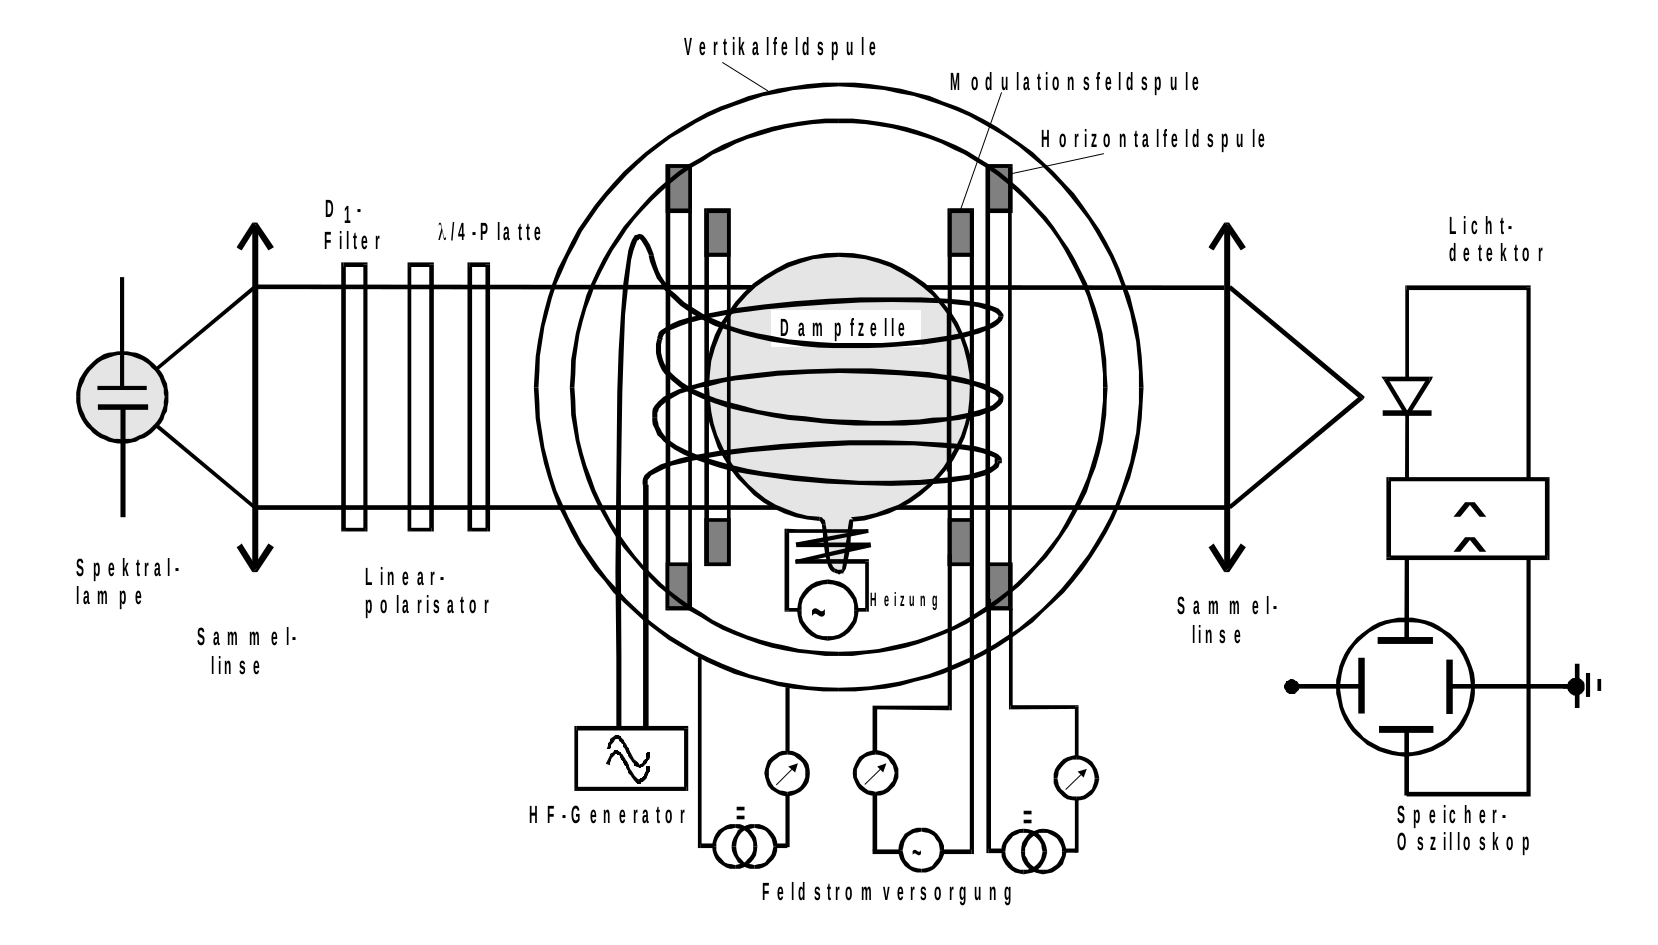
\includegraphics[width=\textwidth]{content/img/aufbau.png}
    \caption{Schematische Darstellung des Versuchaufbaus. \cite{anleitung}}
    \label{fig:aufbau}
\end{figure}
Das Rubidium befindet sich in der Dampfzelle, dessen Temperatur über einen kleinen Ofen gesteuert werden kann.
Um einen optimalen Dampfdruck zu haben wird die Temperatur auf $\qty{50}{\degreeCelsius}$ gehalten.
\\
Wie in \autoref{sec:optisches_pumpen} beschrieben, wird die Probe mit rechtszirkular polarisiertem Licht bestrahlt.
Dazu wird der in der Spektallampe erzeuge Lichtstrahl mit einer Sammellinse gebündelt und trifft anschließend auf den $\text{D}_1$-Filter.
Dieser lässt nur die fürs optisches Pumpen benötigte $\text{D}_1$-Linie ($\lambda = \qty{794.8}{\nano\metre}$) hindurch.
Ein Linearpolarisator filtert dann den nicht-linearpolarisierten Anteil im Licht heraus.
Anschließend wird mit einer $\lambda / 4$-Platte zirkularpolarisiertes Lichts erzeugt, das dann die Rubidiumprobe bestrahlt.
\\
Abhängig von der Transparenz des Rubidiums tritt unterschiedlich viel Licht durch die Dampfzelle hindurch.
Dieses Licht wird mit einer weiteren Sammellinse auf die Photodiode detektiert.
Das erzeugte Signal wird verstärkt und über ein Oszilloskop dargestellt.
\\
Der Aufbau beinhaltet drei Helmholtz-Spulenpaare.
Eine Spule ist vertikal ausgerichtet und soll die vertikalen Komponenten des Erdmagnetfelds kompensieren.
Zwei weitere Helmholtz-Spulen sind horizontal montiert.
Dabei ist eine der Spulen, die sog. \glqq Sweep-Spule\grqq auf der anderen horizontalen Helmholtz-Spule aufgewickelt.
Diese erzeugt über eine festgelegte Zeitperiode und Amplitude ein kontinuierlich ansteigendes Magnetfeld.
\\
Der gesamte Aufbau wird mit einer schwarzen Decke abgedeckt um äußere Einflüsse, insbesondere durch andere Lichtquellen zu reduzieren.
\\
\\
Bevor die Messung beginnen kann, muss das \textbf{Erdmagnetfeld} kompensiert werden.
Der Versuchsaufbau wird so ausgerichtet, dass der Lichtstrahl parallel zur Nord-Süd-Richtung verläuft.
Der longitudinale Anteil des Erdmagnetfelds wird weiter in der Auswertung berücksichtigt.
\\
Der vertikale Anteil soll vollständig durch die senkrechte Spule kompensiert werden.
Dazu wird die Sweep-Spule eingeschaltet.
Auf dem Oszilloskop ist ein Peak zu erkennen.
Dieser tritt auf, wenn die Summe der longitudinalen Magnetfelder null wird.
Die Zeeman-Aufspaltung (siehe \autoref{sec:aufspaltung}) und somit die Besetzungsinversion wird aufgehoben.
Das Rubidium verliert an Transparenz und absorbiert wieder Photonen.
Nun wird durch Modulation der vertikalen Feldstärke die Breite des Peaks minimiert.
\\
\\
Im folgenden wird die \textbf{Resonanzstelle des Magnetfelds} für verschiedene Frequenzen des HF-Feldes gemessen.
Die Resonanz wird für die Frequenzen $\qty{100}{\kilo\hertz}$ bis $\qty{1}{\mega\hertz}$ in $\qty{100}{\kilo\hertz}$-Schritten untersucht.
Dazu wird für jede Frequenz der Strom gemessen an dem die Resonanzstelle des Magnetfelds liegt.
Da das Gasgemisch aus zwei Rubidium-Isotopen besteht existieren auch zwei Resonanzstellen, die beide gemessen werden.
Bei höheren Frequenzen ($~\qty{200}{\kilo\hertz}$) reicht die Magnetfeldstärke der Sweep-Spule nicht aus.
Dann wird die horizontale Spule dazu geschaltet.
Das Gesamtmagnetfeld ergibt sich aus der Summe beider Magnetfelder.
\\
\\
Der Aufbau wird nun angepasst um die Messung zur \textbf{Bestimmung des Verhältnis der Landé-Faktoren der Isotope} durchführen zu können.
Die Sweep-Spule wird zusätzlich an einer Rechteckspannung mit der Frequenz $f=\qty{5}{\hertz}$ angeschlossen.
Es werden $12$ Spannungen im Bereich $\Delta U = [\qty{1}{\volt}, \qty{10}{\volt}]$ untersucht.
Der Strom der Sweep-Spule wird jeweils auf die Resonanzstelle eines Rubidiumisotops eingestellt.
\\
Die Rechteckspannung sorgt dafür, dass im Wechsel der Schwingfall (bzw. Relaxationsfall) und ein Anstieg vorliegt, wo sich das Magnetfeld wieder aufbaut.
\\
Auf dem Oszilloskop wird einmal auf die exponentiell ansteigende Funktion gezoomt.
Die Funktion wird aufgenommen um später Funktionswerte entnehmen zu können.
Zum anderen wird in den Relaxationsbereich gezoomt und die Periodendauer der Schwingung notiert.